%-----------------------------------------------------------------------------%
\chapter{\babDua}
%-----------------------------------------------------------------------------%
Bab ini akan menjelaskan sekilas tentang \textit{computational drug discovery}, apa itu \textit{cloud computing} , dan Docker sebagai platform virtualisasi komputer. 
%-----------------------------------------------------------------------------%
\section{\textit{Computational Drug discovery}}
%-----------------------------------------------------------------------------%
\hspace{0.5cm}\textit{Drug discovery} adalah suatu proses menemukan kandidat obat yang berpotensial. Proses ini melibatkan berbagai displin ilmu seperti biologi, kimia, maupun farmakologi. Dalam \textit{drug discovery} dahulu kala, terkadang obat tersebut ditemukan secara tidak sengaja(\textit{serendipity}) atau berdasarkan penyembuhan tradisional. Seiring dengan berkembangnya pengetahuan dan teknologi, khususnya dalam bidang kimia, ekstraksi senyawa kimia dari makhluk hidup merupakan hal yang wajar. Ekstrak tersebut akan disimpan dan akan disimpan sebagai dalam suatu \textit{library} yang nantinya dapat digunakan kembali. Ekstrak tersebut dapat di-\textit{screening}, apakah terdapat senyawa yang berpotensi sebagai penyembuh dari suatu \textit{sympton} penyakit. Hal ini merupakan dasar farmakologi (\textit{classical pharmacology}).

Waktu yang dibutuhkan dalam proses \textit{drug discovery} cukup lama. Tidak hanya itu, proses ini juga sangat beresiko dan membutuhkan dana yang besar [1].Walaupun demikian, investasi dana dalam \textit{drug discovery} juga berkembang pesat. Namun, investasi tersebut tidak dibarengi dengan hasil yang proporsional dengan investasi tersebut. Hal ini disebabkan oleh rendahnya efektivitas dan tingginya kemungkinan kegagalan dalam \textit{drug discovery}. Beberapa pendekatan telah dilakukan dalam meningkatkan efektivitas, salah satu cara tersebut adalah CADD (\textit{Computer Aided Drug Design}).Dengan begitu, penekanan biaya dan siklus waktu penemuan obat juga semakin cepat. Dalam CADD, komputer digunakan sebagai sarana komputasi dan penyimpanan data dalam \textit{drug discovery}. Tidak ketinggalan, CADD menggunakan aplikasi dalam mendesain ikatan kimiawi, memodelkan struktur kimia yang mengandung kandidat calon obat yang berpotensial dan pembuatan \textit{library} yang dapat digunakan untuk pembelajaran selanjutnya.
\begin{figure}
	\centering
	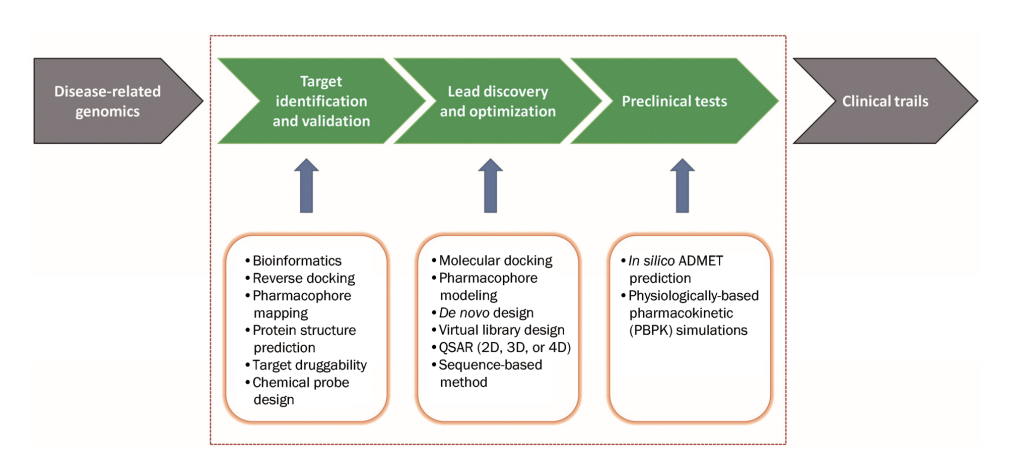
\includegraphics [scale=0.4]{siklus_dd.png}
	\caption{Pemanfaatan komputer sebagai sarana komputasi dalam \textit{drug discovery}}
\end{figure}
Dalam \textit{computational drug discovery} (penemuan obat dengan memanfaatkan komputer), pendekatan yang dapat dilakukan dibagi menjadi \textit{structure-based drug design}(SBDD), \textit{ligand-based drug design}(LBDD) dan pendekatan berdasarkan sekuens.  terdiri dari proses \textit{docking} kandidat \textit{ligand} ke target protein kemudian dilakukan penilaian dengan menggunakan \textit{scoring function} untuk dapat menghitung kemungkinan \textit{ligand}tersebut terikat pada target protein dengan daya tarik yang tinggi. 
\begin{figure}
	\centering
	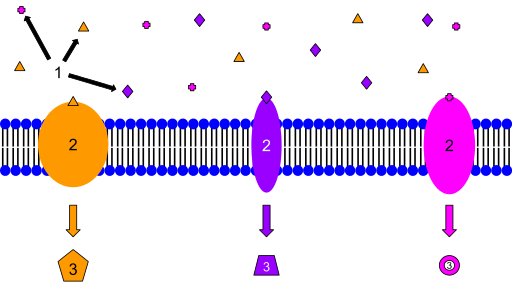
\includegraphics [scale=0.5]{receptor.png}
	\caption{Ilustrasi \textit{ligand}(nomor 1)yang akan terikat dengan \textit{receptor}(nomor 2)}
\end{figure}   
Dalam LBDD, diberikan sekumpulan \textit{ligand} dan \textit{receptor}, dimana model \textit{receptor}dapat dibuat dengan mengumpulkan informasi dari \textit{ligand}. Model ini dikenal dengan \textit{pharmacophore}. Kemudian, kandidat \textit{ligand} akan dibandingkan dengan \textit{pharmacophore}, apakah kompatibel dengan \textit{pharmacophore} dan dapat terikat.
\begin{figure}
	\centering
	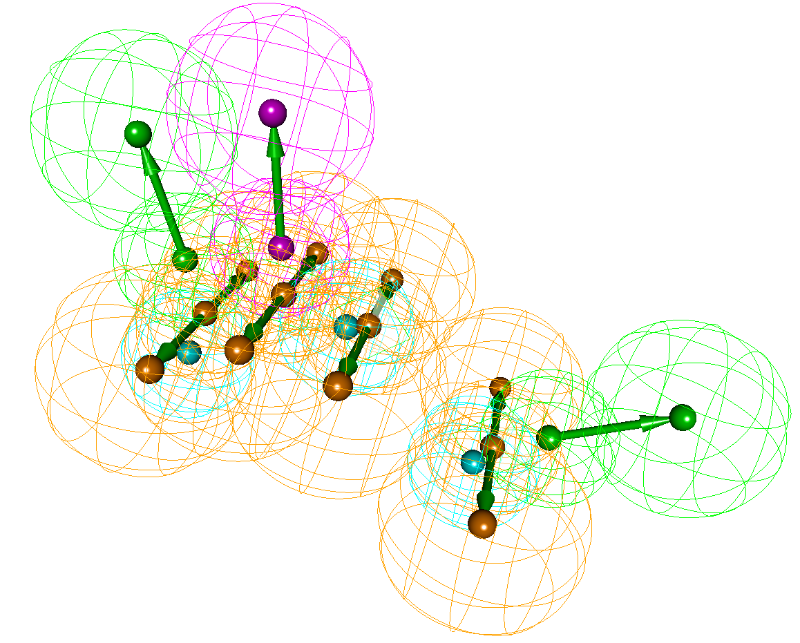
\includegraphics [scale=0.3]{pharmacophore.png}
	\caption{Contoh dari \textit{pharmacophore}}
\end{figure}  

\section{\textit{Molecular Docking}}
%-----------------------------------------------------------------------------%

\textit{Virtual screening} berdasarkan \textit{molecular docking} merupakan metode yang sering digunakan dalam SBDD. Penulis juga akan menggunakan metode tersebut yang terdapat dalam Program Autodock dan Autodock Vina. Pemodelan struktur kimia menggunakan \textit{molecular modeling} untuk mempelajari fenomena dari struktur kimia tersebut. Kemudahan dalam \textit{molecular modeling} sekarang ini dibantu dengan aplikasi komputer yang tersedia, namun masih terdapat kesulitan yaitu bagaiman cara mendapatkan model struktur ikatan kimia yang benar dan interpretasi model yang tepat.Secara umum, \textit{molecular modeling} dapat dikatakan sebagai pemanfaatan komputer dalam mengkonstruksi molekul dan melakukan berbagai macam perhitungan untuk mempelajari karakteristik dan sifat struktur ikatan kimia. Istilah \textit{molecular modeling} terkadang disamakan dengan istilah \textit{computational chemistry}.

Proses \textit{drug discovery} yang semula berupa \textit{trial and error} berubah menjadi proses yang dibantu dengan perhitungan komputer. Perhitungan tersebut digunakan dalam menentukan struktur ikatan kimia baru berdasarkan struktur protein yang sudah diketahui. Pendekatan ini terbagi menjadi dua : \textit{de novo design} dan \textit{docking}. \textit{Docking} merupakan suatu proses untuk menebak struktur \textit{complex} dari struktur \textit{ligand} dan protein. Dalam \textit{molecular modeling}, \textit{docking} dapat dipandang sebagai suatu metode untuk memprediksi orientasi suatu molekul ketika diikat dengan molekul lainnya untuk membentuk \textit{complex} yang stabil.  
\begin{figure}
	\centering
	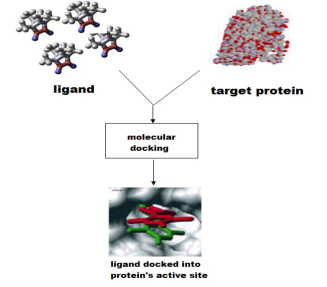
\includegraphics{docking.png}
	\caption{\textit{Proses molecular docking }}
\end{figure}

\textit{Molecular docking} adalah suatu proses komputasi dalam pencarian \textit{ligand} yang paling cocok baik secara geometri maupun energi ketika diikat dengan suatu \textit{receptor}(protein) yang telah diketahui.Aspek utama dalam \textit{molecular docking} adalah perhitungan energi interaksi dan konformasi dengan menggunakan metode dari kuantum mekanik hingga fungsi empiris energi. Permasalahan \textit{molecular docking} sekilas dapat dilihat sebagai suatu permasalahan \textit{lock and key}, dimana \textit{receptor} protein dapat dipandang sebagai \textit{lock} dan \textit{ligand} sebagai \textit{key}. Namun dalam praktiknya, \textit{molecular docking} akan mencari \textit{ligand} yang dapat menyesuaikan dengan \textit{receptor}.karena adaptasi tersebut, \textit{molecular docking} dapat dipandang sebagai permasalahan "\textit{best-fit}" \textit{ligand}. Diperlukan \textit{scoring function} untuk dapat membatasi \textit{best-fit} dari proses \textit{molecular docking}. Fungsi tersebut biasanya berdasarkan \textit{force field} yang digunakan dalam mensimulasikan protein. Beberapa \textit{scoring function} juga menambahkan aspek perhitungan lainnya seperti entropi.
\begin{figure}
	\centering
	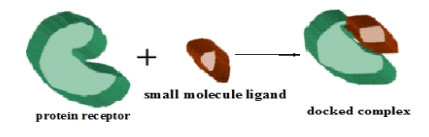
\includegraphics{molecular_docking.png}
	\caption{\textit{best-fit docking}}
\end{figure}
Dalam percobaan ini penulis memanfaatkan aplikasi \textit{molecular docking} Autodock dan Autodock Vina.

\section{\textit{Autodock dan Autodock Vina}}
%-----------------------------------------------------------------------------%
\hspace{0.5cm}Aplikasi ini merupakan aplikasi yang dikembangkan oleh \textit{The Scripps Research Institute}, lembaga riset nonprofit yang terletak di California, Amerika Serikat. Terdapat 2 jenis aplikasi, Autodock dan Autodock Vina. Masing masing merupakan aplikasi yang saling berbeda dalam segi \textit{scoring function} yang digunakan dan optimisasi komputasi secara paralel oleh Autodock Vina. 

Paket aplikasi Autodock terdiri dari 2 program, Autodock4 dan Autogrid4. AutoGrid akan menghasilkan \textit{pre-calculated map} dari suatu \textit{ligand}.Selain itu juga akan menghasilkan \textit{map} tambahan, "d" untuk \textit{desolvation} dan "e" untuk \textit{electrostatic}.Pengoperasian Autodock membutuhkan beberapa file, yaitu : *.dpf untuk pengaturan \textit{docking} parameter , hasil \textit{map} berupa *.gpf dari AutoGrid , dan *.pdbqt untuk \textit{receptor} dan \textit{ligand} yang akan diujicoba. Keluaran yang dihasilkan oleh Autodock berupa *.dlg yang berisi hasil perhitungan konformasi posisi dan energi pada setiap \textit{ligand} yang diujicoba. Paket aplikasi Autodock Vina hanya datang dengan sebuah program saja dikarenakan proses \textit{pre-processing docking} dibuat transparan sehingga pengguna tidak perlu tahu dan memahami bagaimana aplikasi tersebut bekerja. Autodock Vina membutuhkan 2 file, *.pdbqt dari \textit{receptor} dan *.pdbqt dari tiap \textit{ligand} yang akan diujicobakan. Keluaran yang dihasilkan juga beruapa *.pdbqt yang beisikan konformitas posisi dan energi.
\begin{figure}
	\centering
	
\includegraphics{autodock.jpg}
	\caption{Logo Autodock}
\end{figure}

\section{\textit{Cloud Computing}}
%-----------------------------------------------------------------------------% 
\hspace{0.5 cm}Seperti yang telah dijelaskan sebelumnya, pemanfaatan komputer dalam riset mengalami kendala di negara berkembang. Biaya yang harus dikeluarkan dan sumber daya listrik yang dibutuhkan untuk pengadaan \textit{supercomputer} terbilang besar. Selain itu, dibutuhkan pengetahuan lebih terhadap perangkat keras yang akan digunakan tersebut. Hal ini bertujuan supaya pemeliharaan dan penggunaan \textit{supercomputer} lebih baik. Dengan perkembangan teknologi jaringan dan internet yang pesat, muncul teknologi baru yang dikenal dengan \textit{cloud computing}. Teknologi menjawab permasalahan pengadaan perangkat komputasi dan tidak peneliti tidak perlu memahami secara dalam dibalik layanan yang disediakan oleh teknologi tersebut.


\hspace{0.5cm}Teknologi \textit{cloud computing} sudah berkembang sejak tahun 1990-an. Pada awalnya teknologi ini dikembangkan sebagai solusi dari permasalahan yang dihadapi oleh perusahaan dengan bertambahnya kapasitas data yang perlu disimpan dan pengeluaran yang cukup besar untuk pengadaan perangkat keras beserta konsumsi daya listrik yang dibutuhkan. Definisi dari \textit{cloud computing} dapat dikatakan sebagai virtualisasi dari perangkat komputasi, dimana pengguna mengakses perangkat tersebut dengan menggunakan jaringan internet. Selain itu, teknologi ini memberikan kemudahan dalam penggunaan secara \textit{multiuser}, dimana dapat diakses secara bersamaan.

Terdapat 3 karakteristik dari teknologi \textit{cloud computing}, yaitu virtualisasi, terdistribusi, dan kemudahan dalam pengembangan selanjutnya (\textit{dynamically extendibility}). Virtualisasi merupakan faktor yang utama. Virtualisasi dapat membagi suatu perangkat komputasi secara fisik menjadi beberapa "virtual" perangkat komputasi. Dengan begitu, kinerja dari perangkat akan dioptimisasi. Alokasi sumber daya perangkat keras tidak ada yang diam secara percuma. Disamping itu, dengan adanya virtualisasi dapat menekan biaya pengeluaran pengadaan perangkat komputasi secara fisik. Yang dimaksud dengan terdistribusi adalah perangkat keras (\textit{physical node}) yang digunakan dalam \textit{cloud computing} digunakan secara terdistribusi. Dalam tahap pengembangan teknologi ini memberikan kemudahan. Kemudahan tersebut merupakan efek dari virtualisasi. Ketika pengguna ingin mengikuti perkembangan yang ada, tidak perlu merubah / membuat kembali dari awal. Pengguna dapat merubah dari level virtual (virtualisasi).


Terdapat 3 jasa yang disediakan dalam \textit{cloud computing} :
\begin{itemize}
	\item \textbf{Software as a Service (SaaS)}\\
	Layanan jasa ini menyediakan aplikasi dan penyimpanan data (\textit{database}) yang langsung dapat digunakan. Pengguna dapat mengakses aplikasi secara bersamaan dengan pengguna lainnya. SaaS dikenal juga sebagai \textit{on-demand software} dan biaya yang dikenakan oleh penyedia jasa ini merupakan \textit{pay-per-use}. Umumnya, pengguna akan dikenakan biaya bulanan atau tahunan. Pengguna tidak perlu susah - susah untk menginstall aplikasi pada \textit{cloud} dikarenakan penyedia jasa tersebut akan melakukan hal tersebut. Saas memberikan keuntungan bagi perusahaan dengan cara mengurangi biaya operasional IT (Information Technology). Hal ini dikarenakan biaya untuk pemeliharaan dan pengadaan perangkat komputasi ditanggungkan kepada pihak penyedia jasa (\textit{outsourcing}). Contoh dari Saas adalah layanan \textit{e-mail}, media sosial.
	
	\item \textbf{Platform as a Service (PaaS)}\\
	Berbeda dengan Saas, layanan ini menyediakan perangkat komputasi yang dapat digunakan untuk menjalankan aplikasi dari pengguna. Layanan ini dapat menyediakan sistem operasi atau \textit{framework} yang dibutuhkan dalam menjalankan apliksi tersebut. Contoh dari layanan jasa ini adalah : Windows Azure, Amazon Web Service, dan Google App Engine.
	
	\item \textbf{Infrastructure as a Service (IaaS)}\\
	layanan ini menyediakan infrastruktur IT kepada pengguna sesuai dengan permintaan yang dapat diakses dengan jaringan internet. Infrstruktur tersebut meliputi perangkat keras seperti \textit{harddisk, memory, firewall}, tipe server, alamat IP, \textit{virtual local area networks}(VLANs), maupun aplikasi yang harus terinstall dalam server 
	  
\end{itemize}
\begin{figure}
	\centering
	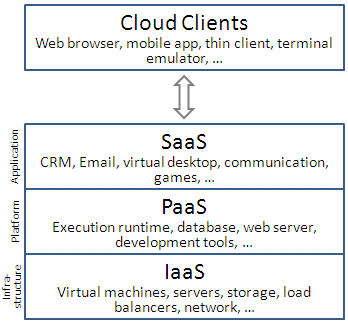
\includegraphics[scale=0.6]{layanan_cloud.png}
	\caption{Layanan dalam \textit{cloud computing}}
\end{figure}